\documentclass[11pt]{article}
\usepackage{mgates-letter}
\definecolor{dark_blue} {rgb}{0., 0., 0.65}
\usepackage{makecell}
\usepackage{listings}
\usepackage{textcomp}
\usepackage{mathrsfs}  % mathscr font
\usepackage{boxedminipage}
\usepackage{rotating}
\usepackage{csquotes}
%\usepackage{natbib}
\usepackage[colorlinks, filecolor=dark_blue, urlcolor=dark_blue, linkcolor=black, citecolor=black]{hyperref}

\begin{document}
\sloppy
\begin{center}
	{{
		\Large{
			\textsc{PhD Programme in Computer Science and Engineering \\ 
			\vspace{4mm}
			Cycle XXXVI}
			}
	}} 
	\rule[0.1cm]{\textwidth}{0.1mm}
	\rule[0.4cm]{\textwidth}{0.6mm}
\end{center}

\begin{center}
	{\LARGE{Engineering Cyber-Physical Swarms with Aggregate Computing}} \\
	\vspace{4mm}
	{\large{PhD Thesis proposal}} 
	\vspace{4mm}
\end{center}
\vspace{8mm}
\par
\noindent
\begin{minipage}[t]{0.47\textwidth}

{\large{Commission: \\\bf
Prof. Mirko Viroli \\
Prof. Andrea Omicini \\
Prof. Matteo Ferrara} 
}
\end{minipage}
\hfill
\begin{minipage}[t]{0.47\textwidth}
	\raggedleft
	{
		\large{PhD Student: \\\bf Gianluca Aguzzi}
	}
\end{minipage}
\vspace{10mm}

{
	\raggedright
	\rule[0.1cm]{\textwidth}{0.6mm}
	\rule[0.5cm]{\textwidth}{0.1mm}
}

\newcommand{\scafiweb}{{ScaFi-Web}}
\newcommand{\scafi}{{ScaFi}}
\newcommand{\cpws}{CPWs}
\newcommand{\rev}[1]{{
	%\color{red}
	#1
	}}
\abstract{
In this thesis aims to define a path towards the engineering of ``Cypher-Physical Swarms" (\cpws) - where swarms are seen in a modern key, including swarm robotics, large-scale IoT scenarios, and crowd engineering (tracking and control). 
%
\cpws are backed by emerging trends of autonomic, pervasive, ubiquitous computing that foster a vision of distributed systems composed of a considerable number of simple entities that collectively perform complex tasks.
%
These systems are similar to natural social-animal groups, where plentiful animals (like ants, sheep, ...) achieve complex tasks (foraging, flocking, ...).
%
Furthermore, these behaviour are typically achieved through self-organisation, making the system robust to failures and highly scalable.
%
Inspired by nature, we define the notion of ``Cypher-Physical Swarm'' -- the extension of `swarms' (of people, of computers, of things) in computer science.
Engineering this kind of system with traditional approaches is inadequate, 
due to the distributed control, high-rate failure, openness, and local-to-global behaviour mapping.
%
Therefore, my thesis is focused on finding a systematic and reproducible way to design \cpws. 
In particular, we plan to leverage Aggregate Computing -- a novel top-down global-to-local programming model.
%
As a final result of my PhD, we intend to analyse the application of Aggregate Computing in \cpws. This will touch on several aspects like distributed intelligence, flexible and opportunistic middlewares, building blocks and ad-hoc DSL.
} %% TODO add discussion on middlewares?? 

\newpage
\tableofcontents
\section{Introduction}
The recent evolution of IT technologies led to a vision in which computation is \textit{everywhere}.
Several modern paradigms advance that vision, like ubiquitous, pervasive, and automatic computing.
%
These consider systems (typically cypher physical) where a large number (thousand - million) of simple interacting devices collectively perform complicated tasks in a decentralised manner, acting and sensing through a shared environment. 
%
Thus, they can be conceived as \textit{complex} systems like the one observed in nature --  by means that we cannot understand the behaviour of the whole looking only at the parts.
%
Speaking about natural systems, social animals, like a swarm of insects, exhibit fault-tolerant, effective, and efficient collective behaviours leveraging self-organisation.

Hence we want to promote cypher-physical systems with the properties observed in swarms. 
%
Therefore we lead to define Cypher-Physical-Swarm (\cpws): a collection of (simple) computational entities linked with the physical world via perception and actuation that reach collective goals through self-organising behaviours.
%
Swarm robotics, ``swarms” of people (crowds) or, in general, ``swarms” of IoT devices are clearly defined instances of \cpws.

Traditional design methodologies are inadequate for \cpws engineering, due to local-to-global mapping problems, distributed control, complex IT infrastructures and scalability concerns.
%
Following this line, the goal of my research PhD thesis is to find a systematic methodology (models, techniques and algorithms)
to synthesise and deploy self-organising behaviours of predictable outcomes for \cpws.

This is not the first effort in this direction. Indeed, traditionally, designers have been guided
by natural phenomena observation that was then transposed into computer systems -- a so-called
bottom-up approach. 
%
However, this trend led to specific solutions that hardly scale up with application complexity.
Novel techniques -- and the one that we follow in this work -- consist of a top-down global-to-local approach where designers define the system outcome directly at the collective level. 
%
Among the many (like Buzz, TOTA) in this thesis, we will take into consideration Aggregate Computing since it enables the definition of self-organising collective behaviour through the manipulation of a distributed data structure called computational field.
%
In this way, the program specification is “collectively” declared, abstracting over underlying aspects – such as network topology or communication protocol – and making it applicable to any system size. 

Even if Aggregate Computing is applied already in different scenarios like crowds of people, smart cities, and large-scale IoT, it currently lacks software architecture (middleware), systematic program definition, abstraction layers (DSL) and foundational aspects.
%
Consequently, my thesis aims to investigate and analyse critically Aggregate
Computing techniques in the field of \cpws. 
%
This investigation will address multiple directions
like distributed intelligence, flexible middlewares, and ad-hoc building blocks, possibly leading to contributions both at a foundational (i.e. building blocks, aggregate computing language,  DSL) and ``architectural" level (middleware, message passing architecture, ...).
%
In this process, Machine Learning techniques could be used in support of Aggregate Computing to enhance adaptivity

The proposal is then structured as follow. In \Cref{background} I discuss the current state-of-the-art methodologies and related works in the field \cpws behaviour definition.
%
In \Cref{contribution} I devise my thesis contribution in the path of engineering predictable outcome in \cpws. Furthermore, I show my preliminary works done in my first PhD year and the future works that I plan to do. 


\section{Background} \label{background}
%%% Expand the discussion of cpws, specilizing it against other scenarion
%% So the properties are: partial observability, no centralized entity, an overall behaviour similar to what is seen in swarm ==> all the thins linked with swarm like system.
\subsection{Multi-Agent Systems}
A CPSWs could be seen as multi-agent system and, often, a \emph{many}-agent system where a large number (hundreds or more) of autonomous entities are programmed to achieve some collective behaviour through \emph{repeated}  sensing, computation, communication, and actuation steps.

Due to the high stochasticity of the environment, it is almost impossible to know and program the optimal behaviour for all agents in advance.
%  
This uncertainty results in the need of creating intelligent agents so that they can learn the optimal behaviour and adapt to environmental changes.
\subsubsection{Learning}
In recent decades there has been an emerging trend in the use of RL 
in multi-agent settings -- called Multi-Agent Reinforcement Learning (MARL) -- as a powerful, robust and adaptive learning paradigm.
%
Progress has been considerable and a wide range of algorithms are now available.

MARL is a conjunction of Game theory and RL, 
 and there are several (even orthogonal) viewpoints on which researchers have been focused.

First attempts from RL viewpoint, 
 goes towards a so-called \textit{independent learning}~\cite{DBLP:journals/tsmc/BusoniuBS08} approach, 
 where each agent learn locally against the whole environment~\cite{DBLP:conf/icml/Tan93}.

Examples of these are Hysteretic Q-Learning (used to reduce non-stationarity)~\cite{hysteretic-q}, 
 Lenient Learning~\cite{DBLP:journals/jmlr/WeiL16}, and Frequency Maximum Q-value~\cite{DBLP:conf/atal/KaisersT10}.
%
The pro of these approaches is that their complexity does not scale up with the number of agents, 
 but, unfortunately, the learning process is extremely non-stationary and unstable.
% 
Furthermore, they are heuristic and do not exist any convergence proof (even if, in practice, they often reach a good policy).

Other efforts have focussed on achieving equilibria such as Nash-equilibrium of Pareto optimality.
 The first works towards this direction are Nash-Q-Learning~\cite{nash-q}, Friend-or-Foe Q-learning~\cite{DBLP:conf/icml/Littman01}, Minimax-Q~\cite{DBLP:conf/icml/Littman94}.
The problem is that it is used with few agents and scale hardly with the application complexity.
%
Finally, current emerging trends tend to leverage a so-called centralised training and decentralised execution (CTDE) approach, by which 
 agents should leverage the system-wide knowledge at training time but at runtime, they act independently~\cite{DBLP:journals/aamas/Hernandez-LealK19}.
 Most promising approaches in this direction are MAPPO~\cite{DBLP:journals/corr/abs-2103-01955}, COMA~\cite{DBLP:journals/corr/FoersterFANW17} and MADDPG~\cite{DBLP:conf/nips/LoweWTHAM17}.
 
The main problem with most of the solutions available in the literature is that they consider a small number of agents (or at least test them on small games).
 In AC instead, we need to find a technique that does not depend on the system node count.
\subsection{Aggregate Computing}

Aggregate computing is an approach to specify or \emph{self-organising} behaviour of a MAS from a global perspective.
%
The aggregate program (i.e. a program written with aggregate computing) provides a way to map the local observations of an individual agent (i.e., sensing information, current agent state, and inbound messages from neighbours) to (eventually) globally-coherent local actions
 (i.e., actuation instructions, and outbound messages).
%

Historically, aggregate programming originated from works drawing inspiration from nature: whereas the biological inspiration led to swarm intelligent MASs, where agent indirectly interact by pheromones \cite{DBLP:conf/atal/ParunakBS02}, the physical inspiration led to the idea of agents acting in environments empowered with potential fields \cite{DBLP:books/daglib/0015276}.
%
Recently, aggregate programming has been formally backed by \emph{field calculi}~\cite{viroli2019jlamp-si-coord}, which provide a compositional approach
 to global behaviour specification
 based on functions from fields to fields.
%
A \emph{(computational) field} is a map associating a value to any device of a given domain.
%
So, for instance, controlling the movement of a swarm of drones can be expressed through a field of velocity vectors, which maps any drone of the swarm to a corresponding velocity (speed and direction); the set of low-energy devices can be denoted through a Boolean field holding \texttt{true} for devices whose local energy level (as perceived by local sensors, and collectively also denoted as a floating-point field) is under a certain threshold (also a floating-point field).
%
These fields, then, are generally manipulated through three kinds of constructs:
\begin{enumerate}
\item \emph{Stateful evolution}: \lstinline|rep(init)(f)|---expressing how a field, starting as \lstinline|init|, should evolve round-by-round through unary function \lstinline|f|.
\item \emph{Neighbour interaction}: \lstinline|nbr(e)|---used to exchange with neighbours the value obtained by evaluating field expression \lstinline|e|; this locally yields a \emph{neighbouring field}, i.e., a field that maps any neighbour to the corresponding evaluation of \lstinline|e|.
\item \emph{Domain partitioning}: \lstinline|branch(c){ifTrue}{ifFalse}|---used to partition the domain of devices into two parts: the devices for which field \lstinline|c| is locally \lstinline|true|, which evaluate expression \lstinline|ifTrue|, and those for which \lstinline|c| yields \lstinline|false|, which evaluate \lstinline|ifFalse|. 
\end{enumerate}
%
The idea of aggregate programming is to 
 write programs talking about global behaviour (fields)
 and let these drive the local activity of every device in the system.
%
Aggregate programming is embodied by concrete aggregate programming languages~\cite{viroli2019jlamp-si-coord},
 such as ScaFi~\cite{DBLP:conf/isola/CasadeiVAD20,DBLP:journals/eaai/CasadeiVAPD21},
 a Domain-Specific Language (DSL) embedded in Scala
 as well as a toolchain for aggregate system development and simulation~\cite{Casadei2016mass}.
%

As target tooljit, we probably adopt ScaFi in this my thesis work mostly for practical reasons: with respect to other aggregate programming languages such as Proto and Protelis, surveyed in \cite{viroli2019jlamp-si-coord},
ScaFi is a \emph{strongly typed}, \emph{internal} DSL; therefore, it enables straightforward reuse of powerful features from the Scala host language (including its type system, type inference, programming abstractions, libraries).

Additionally, ScaFi also represents an agile framework for testing experimental language features (cf. \emph{aggregate processes}~\cite{DBLP:journals/eaai/CasadeiVAPD21}.
%
Hence, among the existing languages for aggregate programming, we believe ScaFi is the one better fitting rich scenarios like what we expected for \cpws.

A full account of research about aggregate programming, field calculi, and ScaFi is beyond the scope of this proposal; more details can be found in~\cite{viroli2019jlamp-si-coord,DBLP:journals/eaai/CasadeiVAPD21}.

\section{Contribution} \label{contribution}
\subsection{Thesis proposal}
\begin{figure}
	\centering
	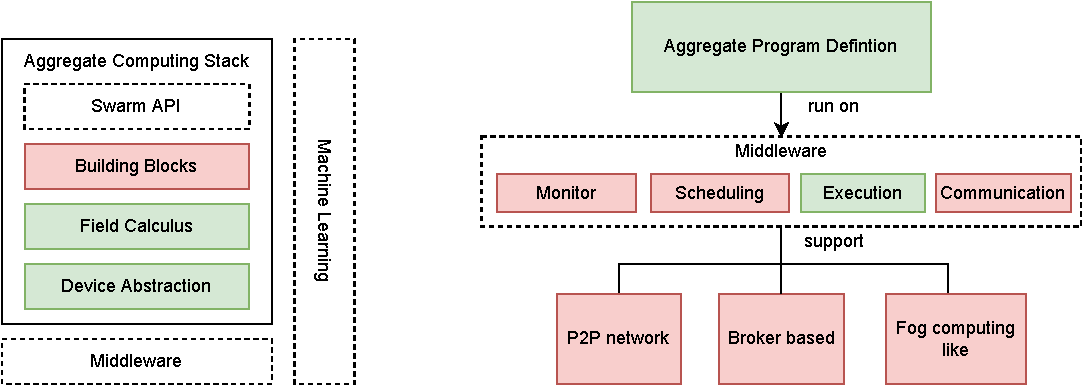
\includegraphics[width=\textwidth]{img/to-do-for-thesis.pdf}
	\caption{Devise the current status of aggregate computing toolkit in literature. Dotted blocks mean a lack of that concept. Green block are the one that can be consider stable and reusable in \cpws engineering. Red Block are the one that currently exists but need to be expanded in order to support \cpws.}
	\label{fig:current-state}
\end{figure}
My PhD thesis will be focused on the engineering process of \cpws leveraging Aggregate Computing abstractions. The choice of Aggregate Computing as a conceptual model for describing \cpws behaviours is well fitted since it:
\begin{itemize}
	\item Allows defining collective behaviour failure robust and scale-independent: the aggregate programs are expressed through manipulation of computational field, abstracting over nodes itself and treating the systems like a computational blob that evolves in time. In doing that, the logic is independent of the node population, so it handles natively failure, openness and the same program can be applied to very dense IT networks.
	\item Enhances the possibility to \textit{program} self-organisation: Typically, self-organisation is something that was achieved by observing natural phenomena. Aggregate Computing wants to give a systematic way to let \textit{self-organising} behaviour programmable. To do that, the programs are defined using a composition of building blocks that expose self-organising patterns.
	\item Is applicable to different deployment kinds leveraging modern complex IT infrastructures: Aggregate program does not depend on any particular IT network framework. Potentially, it could be applied in cloud-like systems, P2P networks and client and server architecture (the direction of pulverisation). This is particularly important for \cpws since they could leverage different kinds of networks.
\end{itemize}

This choice impact strongly on the design process of collective application. Some of the concerns are already tackled in related words but others are currently quite unexplored and for us are essential in the context of CPWS, and this is where my thesis work will be focused on.
In particular, the main concerns where my work is placed are:
\begin{itemize}
	\item Development of \textit{flexible} middleware: In this year, the main effort of this line of the research concern \textit{foundational} aspects. However, currently, little effort is done to make aggregate programs applicable to various deployment kinds. Furthermore, we would like to leverage current IT infrastructures opportunistically (like edge computing or osmotic computing). In this line, in my thesis, I would produce software artefact in order to \textit{support} such kind of middleware for \cpws.
	\item Building blocks definition from \cpws: During the study and the analysis of CPSWs, we would encounter the possibility of describing new building blocks. For instance, in swarms the concept of \emph{cluster} is central for several reasons: identifying a group of entities with common capabilities, we can use it to produce a mean view of a certain zone, and so on. Therefore, we probably need to enlarge the current building block set to new constructs, that possibly could be useful also to other scenarios (like smart cities, smart grid, ...).
	\item Definition of API for swarm-like behaviour: Aggregate Computing is based on a layered approach. Typically, for each different scenario, developers should define an API to support a particular kind of application. So, in this thesis, we will focus on the definition of common abstraction needed to program \cpws.
	\item Improvements of the entire Aggregate Computing stack with Machine Learning: Aggregate computing stack concern different aspects, from API to field-calculus to middleware. Machine Learning -- and in particular Reinforcement Learning -- in this context could be used as an intrinsic mechanism to improve adaptivity.
\end{itemize}

\subsection{Preliminary contributions}
In my first year of PhD, my activities have been centred on
the integration of Aggregate Computing with Machine Learning capability to create even more
intelligent collective behaviour. 

My work climaxes with ~\cite{research} where I explain different suitable approaches to
enhance Aggregate Computing with Machine learning. Finally, in the last period, I made concrete
experiments with Reinforcement Learning -- in particular, Q-Learning \cite{} -- improving the current Aggregate Computing solutions.

Concerning middleware aspects, my research activities aim at closing the gap between
its abstract space and its application in concrete systems. In this direction, I made mainly contributions to \scafi. In particular, we produce two articles concerning ScaFi-Web -- a web-based tool that could support monitoring aspects and \scafi Loci -- a type-safe deployment methodology leveraging multi-tier programming.
\subsubsection{ScaFi-Web -- A tool for a distributed monitoring}
\scafiweb{}\footnote{\url{https://scafi.github.io/web}}
 is an online playground for learning aggregate computing, experimenting with it, and monitoring executions in a browser.
% a  web-based platform supporting \scafi{} in-browser that
It currently features:
\begin{itemize}
 \item an interactive editor for writing \scafi{} programs;
 \item a guided tour of the most prominent features, kickstarting development;
 \item an in-browser simulated network of devices hosting the execution;
 \item visualisation, inspection, and interaction tools integrated with the simulated environment.
\end{itemize}

Furthermore, it also provides a stepping stone towards a monitoring and control system for aggregate computing deployments.

Indeed, In the context of field-based coordination, automated runtime verification approaches have been recently investigated, whereby spatial or temporal logics are mapped to field calculus programs to directly encode the behaviour of decentralised monitoring.

The \scafiweb{}'s frontend has been designed to be adaptable to different backends; indeed, the UI is completely separated from the underlying aggregate execution system. 

\subsubsection{ScaFi Loci -- Towards a type-safe deployment of Pulverised Architecture}
Aggregate computing defines a conceptual model by which is possible to define collective computation. Practically, each node needs to have a notion of the neighbourhood (i.e what nodes are near to me) following a certain metric. \textit{How} this neighbourhood is built, is transparent for the computational model. Therefore it is possible to deploy the same application in different IT networks.

Pulverised architectures (i.e. pulverisation) go in this direction, identifying the main \textit{deployable} units that can be moved in different concrete nodes, the core idea is that the functional
the behaviour of a distributed application is fundamentally orthogonal to the actual deployment of the services that compose it.

However, pulverisation does not specify how a pulverised architecture should
be described and verified so that it can be operated correctly
at runtime.
Therefore, in \scafiweb Loci we define an architecture for multitiered deployment strategies in pulverised systems, along with an implementation using ScaFi and ScalaLoci.

The latter enables a \textit{typesafe} multitier programming approach -- by which distributed architecture is defined
in a single compilation unit with a single language.

This work could be seen as a piece of the flexible middleware that we intend to build, focused only on the deployment aspects.

\subsection{Future works}

\subsubsection{Swarm API}
The thesis will extend the current aggregate computing stack with high-level API about swarms behaviours (Swarm API) like flocking, foraging, blinking and spreading of information.  Consequently, self-adaptive properties have to be verified as done in other building blocks.  The swarm API will not only mimic some nature-inspired behaviours, but it will give a general interface to solve common collective problems. The API could be reused under the general collective adaptive system (CAS) context.
\subsubsection{Improve to speed up convergence: Machine Learning applied to Building Blocks}
Aggregate Computing based its logic in \textit{compositionality} inspired by functional programming. The idea is that complex behaviours can be defined only through the composition of \emph{building blocks}. Furthermore, based on these programming bricks, relevant collective properties are proven such as self-stabilization and eventual consistency. 

Currently, the key problem with those building blocks is that they aren't able to be used in any kind of network topology. Indeed we are dealing with high node dynamic, the overall computation field became quite a noise and unstable -- leading to ever reaching our intended result.

Traditionally these problems are tackled with heuristic/algorithmically to solve various problems (stability of results, convergence speed up, ...). But this led to complex fine-tuning and algorithm choice for each new environment.

Our idea hypothesis in~\cite{research} consists of applied Machine Learning algorithms -- and in particular Reinforcement Learning -- to improve building blocks by means of speeding up the self-stabilisation process.
\subsubsection{Middleware-level learning}
%% Talk about the aspect of time fuild (distributed scheduler) and space fluid (discard message opportunistically).
\subsection{Evaluation}\label{evaluation}
The current development process

\bibliographystyle{ieeetr}
\bibliography{biblio}

\end{document}
